\documentclass[12pt,letterpaper]{amsart}
\setlength{\oddsidemargin}{.0in}
\setlength{\evensidemargin}{.0in}
\setlength{\textwidth}{6.5in}
\setlength{\topmargin}{-.3in}
\setlength{\headsep}{.20in}
\setlength{\textheight}{9.in}
\usepackage[leqno]{amsmath}
\usepackage{amsfonts}
\usepackage{amssymb}
\usepackage{amsthm}
\usepackage{amssymb}
\usepackage[all]{xy}
\usepackage{graphicx}



%Here are some user-defined notations
\newcommand{\RR}{\mathbf R}
\newcommand{\CC}{\mathbf C}
\newcommand{\ZZ}{\mathbf Z}
\newcommand{\ZZn}[1]{\ZZ/{#1}\ZZ}
\newcommand{\QQ}{\mathbf Q}
\newcommand{\rr}{\mathbb R}
\newcommand{\cc}{\mathbb C}
\newcommand{\zz}{\mathbb Z}
\newcommand{\zzn}[1]{\zz/{#1}\zz}
\newcommand{\qq}{\mathbb Q}
\newcommand{\calM}{\mathcal M}
\newcommand{\latex}{\LaTeX}
\newcommand{\tex}{\TeX}
\newcommand{\sm}{\setminus} 


%improving spacing in tables (space above and below characters in a row)
\newcommand{\tfix}{\rule{0pt}{2.6ex}}
\newcommand{\bfix}{\rule[-1.2ex]{0pt}{0pt}}



%Here are commands with variable inputs 
\newcommand{\intf}[1]{\int_a^b{#1}\,dx}
\newcommand{\intfb}[3]{\int_{#1}^{#2}{#3}\,dx}
\newcommand{\marginalfootnote}[1]{%
        \footnote{#1}
        \marginpar[\hfill{\sf\thefootnote}]{{\sf\thefootnote}}}
\newcommand{\edit}[1]{\marginalfootnote{#1}}


%Here are some user-defined operators
\newcommand{\Tr}{\operatorname {Tr}}
\newcommand{\GL}{\operatorname {GL}}
\newcommand{\SL}{\operatorname {SL}}
\newcommand{\Prob}{\operatorname {Prob}}
\newcommand{\re}{\operatorname {Re}}
\newcommand{\im}{\operatorname {Im}}


%These commands deal with theorem-like environments (i.e., italic)
\theoremstyle{plain}
\newtheorem{theorem}{Theorem}[section]
\newtheorem{corollary}[theorem]{Corollary}
\newtheorem{lemma}[theorem]{Lemma}
\newtheorem{conjecture}[theorem]{Conjecture}

%These deal with definition-like environments (i.e., non-italic)
\theoremstyle{definition}
\newtheorem{definition}[theorem]{Definition}
\newtheorem{example}[theorem]{Example}
\newtheorem{remark}[theorem]{Remark}

%This numbers equations by section
\numberwithin{equation}{section}

\begin{document}
\begin{definition}(\textbf{Brownian Motion}) is a stochastic process that models random continuous motion. The stochastic process $B=\{B(t), t\geq 0\}$ is standard Brownian Motion if the following holds:
\begin{enumerate}
\item[(1)]
$B$ has independent increments.
\item[(2)]
For $0 \leq s < t,$ $$B(t)-B(s) \sim N(0,t-s),$$\\
meaning the increment $B(t)-B(s)$ is normally distributed with mean $0$ and variance equal to the lenth of the increment separating $s \ \text{and} \ t$
\item[(3)] With probability $1$, paths of $B$ are continuous; that is, $$P[B \in C[0, \infty)]=1.$$
\item[(4)] $B(0)=0$ 
\end{enumerate}
\end{definition}

The Brownian motion process, sometimes referred to as the Weiner process can be thought of as a continuous time approximation of a random walk where the size of the steps is called to become smaller and the rate at which steps are taken is speeded up. \\


******INSERT RANDOM WALK SIMULATION HERE???*****

\begin{definition}(\textbf{Markov Process}) is a stochastic process with the following properties: 
\begin{enumerate}
\item[(a.)] The number of possible outcomes or states if finite
\item[(b.)] The outcome at any stage depends only on the outcome of the previous stage.
\item[(c.)] The probabilities are constant over time.   
\end{enumerate}

\begin{example}
$$ \frac{x(\lambda t)}{\sqrt{\lambda}}$$ is a Brownian motion. 
\begin{proof}
\begin{align*}
 & \frac{x(\lambda t)}{\sqrt{\lambda}}-\frac{x(\lambda s)}{\sqrt{\lambda}}\\
 & P \left(a \leq \frac{x(\lambda t)}{\sqrt{\lambda}}-\frac{x(\lambda s)}{\sqrt{\lambda}} \leq b \right)=P \left(a \sqrt{\lambda} \leq x(\lambda t) - x (\lambda s) \leq b \sqrt{\lambda} \right)\\
 & \displaystyle \frac{1}{\sqrt{2 \pi (\lambda t -\lambda s)}} \int_{a \sqrt{\lambda}}^{b \sqrt{\lambda}} e^{\frac{-x^2}{2}(\lambda t- \lambda s)} dx\\
  & u=\frac{x}{\sqrt{\lambda}}\\
  & du=\frac{1}{\sqrt{\lambda}}\\
  & =\frac{1}{\sqrt{2 \pi \lambda(t-s)}} \int_{a}^{b} e^{\frac{-u^2}{t-s}} \cdot \sqrt{\lambda}du\\
  & = \frac{1}{\sqrt{2 \pi (t-s)}} \int_{a}^{b} e^{\frac{-u^2}{t-s}}du
 \end{align*}
 \end{proof}

Brownian motion because has a $\mu=0 \ \text{and} \ \sigma^2=t-s$
\end{example}

\end{definition}

(\textbf{Riemann-Stieltjes Integral}): 
$$\displaystyle \int_{a}^{b} f(g)dg= \underset{n \to \infty}{\lim} \sum_{i=1}^{N} f(g(t_i)) \cdot (g(t_{i+1}))- g(t_i))$$\\

The main motivation for the Riemann-Stieltjes Integral comes from the concept of Cumulative Distribution Function (CDF) of a random variable. 

\textbf{Weiner Integral} $$\int_{a}^{b} f(t)dW(t)$$
$$1[t_{i+1}, t_i] (t)= \begin{cases} 1 & \text{if} \ t_{i+1} \leq t < t_i \\
0 & \text{otherwise} \end{cases}$$

\textbf{Multivariate Taylor Expansion:} $$F(t)-F(s)=F^{\prime}(s)(t-s)+\frac{1}{2}F^{''} (s)(t-s)^2 + \frac{1}{3!}F^{'''}(t-s)^3+ \text{H.O.T}$$

\textbf{It\^{o}'s Formula} $$\displaystyle F(t, B(t))-F(a,B(a))= \int_{a}^{t} \frac{\partial F}{\partial s}ds+ \int_a^t \frac{\partial F}{\partial B} dB+ \delta t+ \int_a^t \frac{1}{2} \frac{\partial^2 F}{\partial B^2} ds$$

\begin{example}
Let $F=tB^2$ 
\begin{align*}
\displaystyle
&\frac{dF}{dt}= B^2\\
&\frac{dF}{dB}=2t+B\\ 
&\frac{d^2 F}{dB^2}=2t
\end{align*}
\begin{align*}
tB^2(t)-aB^2(a) &=\int_{a}^{t}B^s ds+ \int_{a}^{t}2sBdB+\int_a^t \frac{1}{2}2sds\\
 &=\int_a^b B^2+sds+\int_a^t 2sBdB\\
 &\text{OR}\\
tB^2(t)-aB^2(a) &= \int_a^t B^s ds+ \int_a^t 2sBdBt+ \frac{1}{2} t^2- \frac{1}{2}a^2
\end{align*}
\end{example}

\begin{example} Use It\^o's formula to find an integral expression for the following integraL:
$$f(B)=B^4$$
\begin{align*}
f(x)&=B^4\\
f'(x)&=4B^3\\
f''(x)&=12B^2\\
d(B^4)&= 4B^3(t)dB+\frac{1}{2}(12B(t)^2)dt\\
	&=4B^3(t)dB+6B^2(t)dt\\
B^4(t)&= 4 \int_0^t B^3 dB+ 6 \int_0^t B^2 ds\\
E\left[\int_0^t B_s^2 ds\right] &= \frac{1}{6}E \left[B_t^4-4 \int_0^tB_s^3 dBs \right]\\
 &=\frac{1}{6}  \left[E \left[B_t^4\right]-4E\left[\int_0^t B_s^3 dBs \right] \right]\\
 &=\frac{1}{6}(3t^2)
\end{align*}
\end{example}

\textbf{Nondimensionalization}: method to reduce parameters. 

\begin{enumerate}
\item
List all the variables and parameters along with their dimensions.
\item
For each variable, say $x$, form a product (or quotient) $p$ of parameters that has the same dimensions as $x$, and define a new variable $y=\frac{x}{p}.$ $y$ is a "dimensionless" variable. It's numberical  value is the same no matter what system of units is used.
\item Rewrite the differential equation in terms of the new variables.
\item 
In the new differential equation, group the parameters into nondimensional combinations, and define a new set of nondimensional parameters expressed as the nondimensional combinations of the original parameters. 
\end{enumerate}

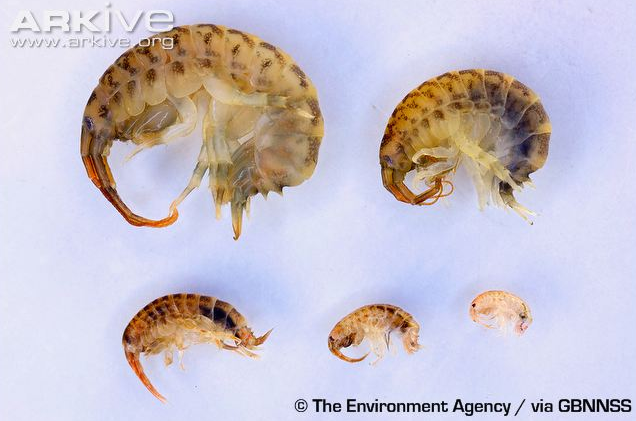
\includegraphics[scale=.75]{shrimpy1}\\


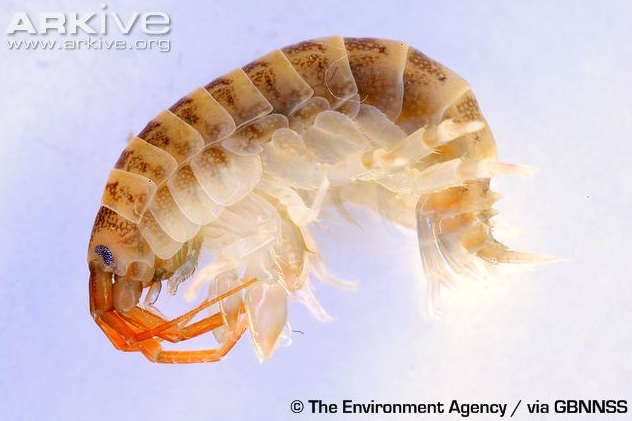
\includegraphics[scale=.75]{shrimpy2}\\

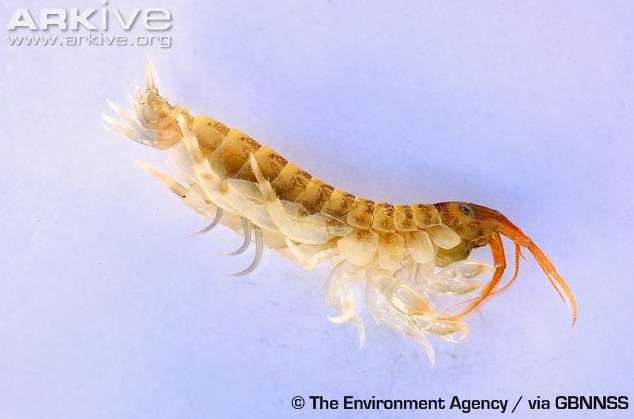
\includegraphics[scale=0.75]{shrimpy3}



\end{document}

